\documentclass[a4paper,12pt]{article}
\usepackage[utf8]{inputenc}
\usepackage[margin=1in]{geometry}
\usepackage{parskip}
\usepackage{graphicx}
\usepackage{hyperref}
\usepackage{listings}
\usepackage{multirow}
\hypersetup{colorlinks}
\lstset{basicstyle=\ttfamily}

\title{Data Structures and Algorithms 120:\\Inventory Assignment Report}
\date{October 7, 2013}
\author{Delan Azabani}

\begin{document}

\maketitle

\pagenumbering{arabic}

\section{Known defects}

The application allows the user to build a binary search tree regardless of
whether or not the array has been sorted due to the invocation of the ``Save
data to file'' function. Doing so after the data is output to a file will cause
a degenerate tree to be built, which is extremely inefficient. I chose not to
manually prevent this to allow a live comparison of the two scenarios,
demonstrating the importance of using a randomised input array.

\section{UML class diagram}

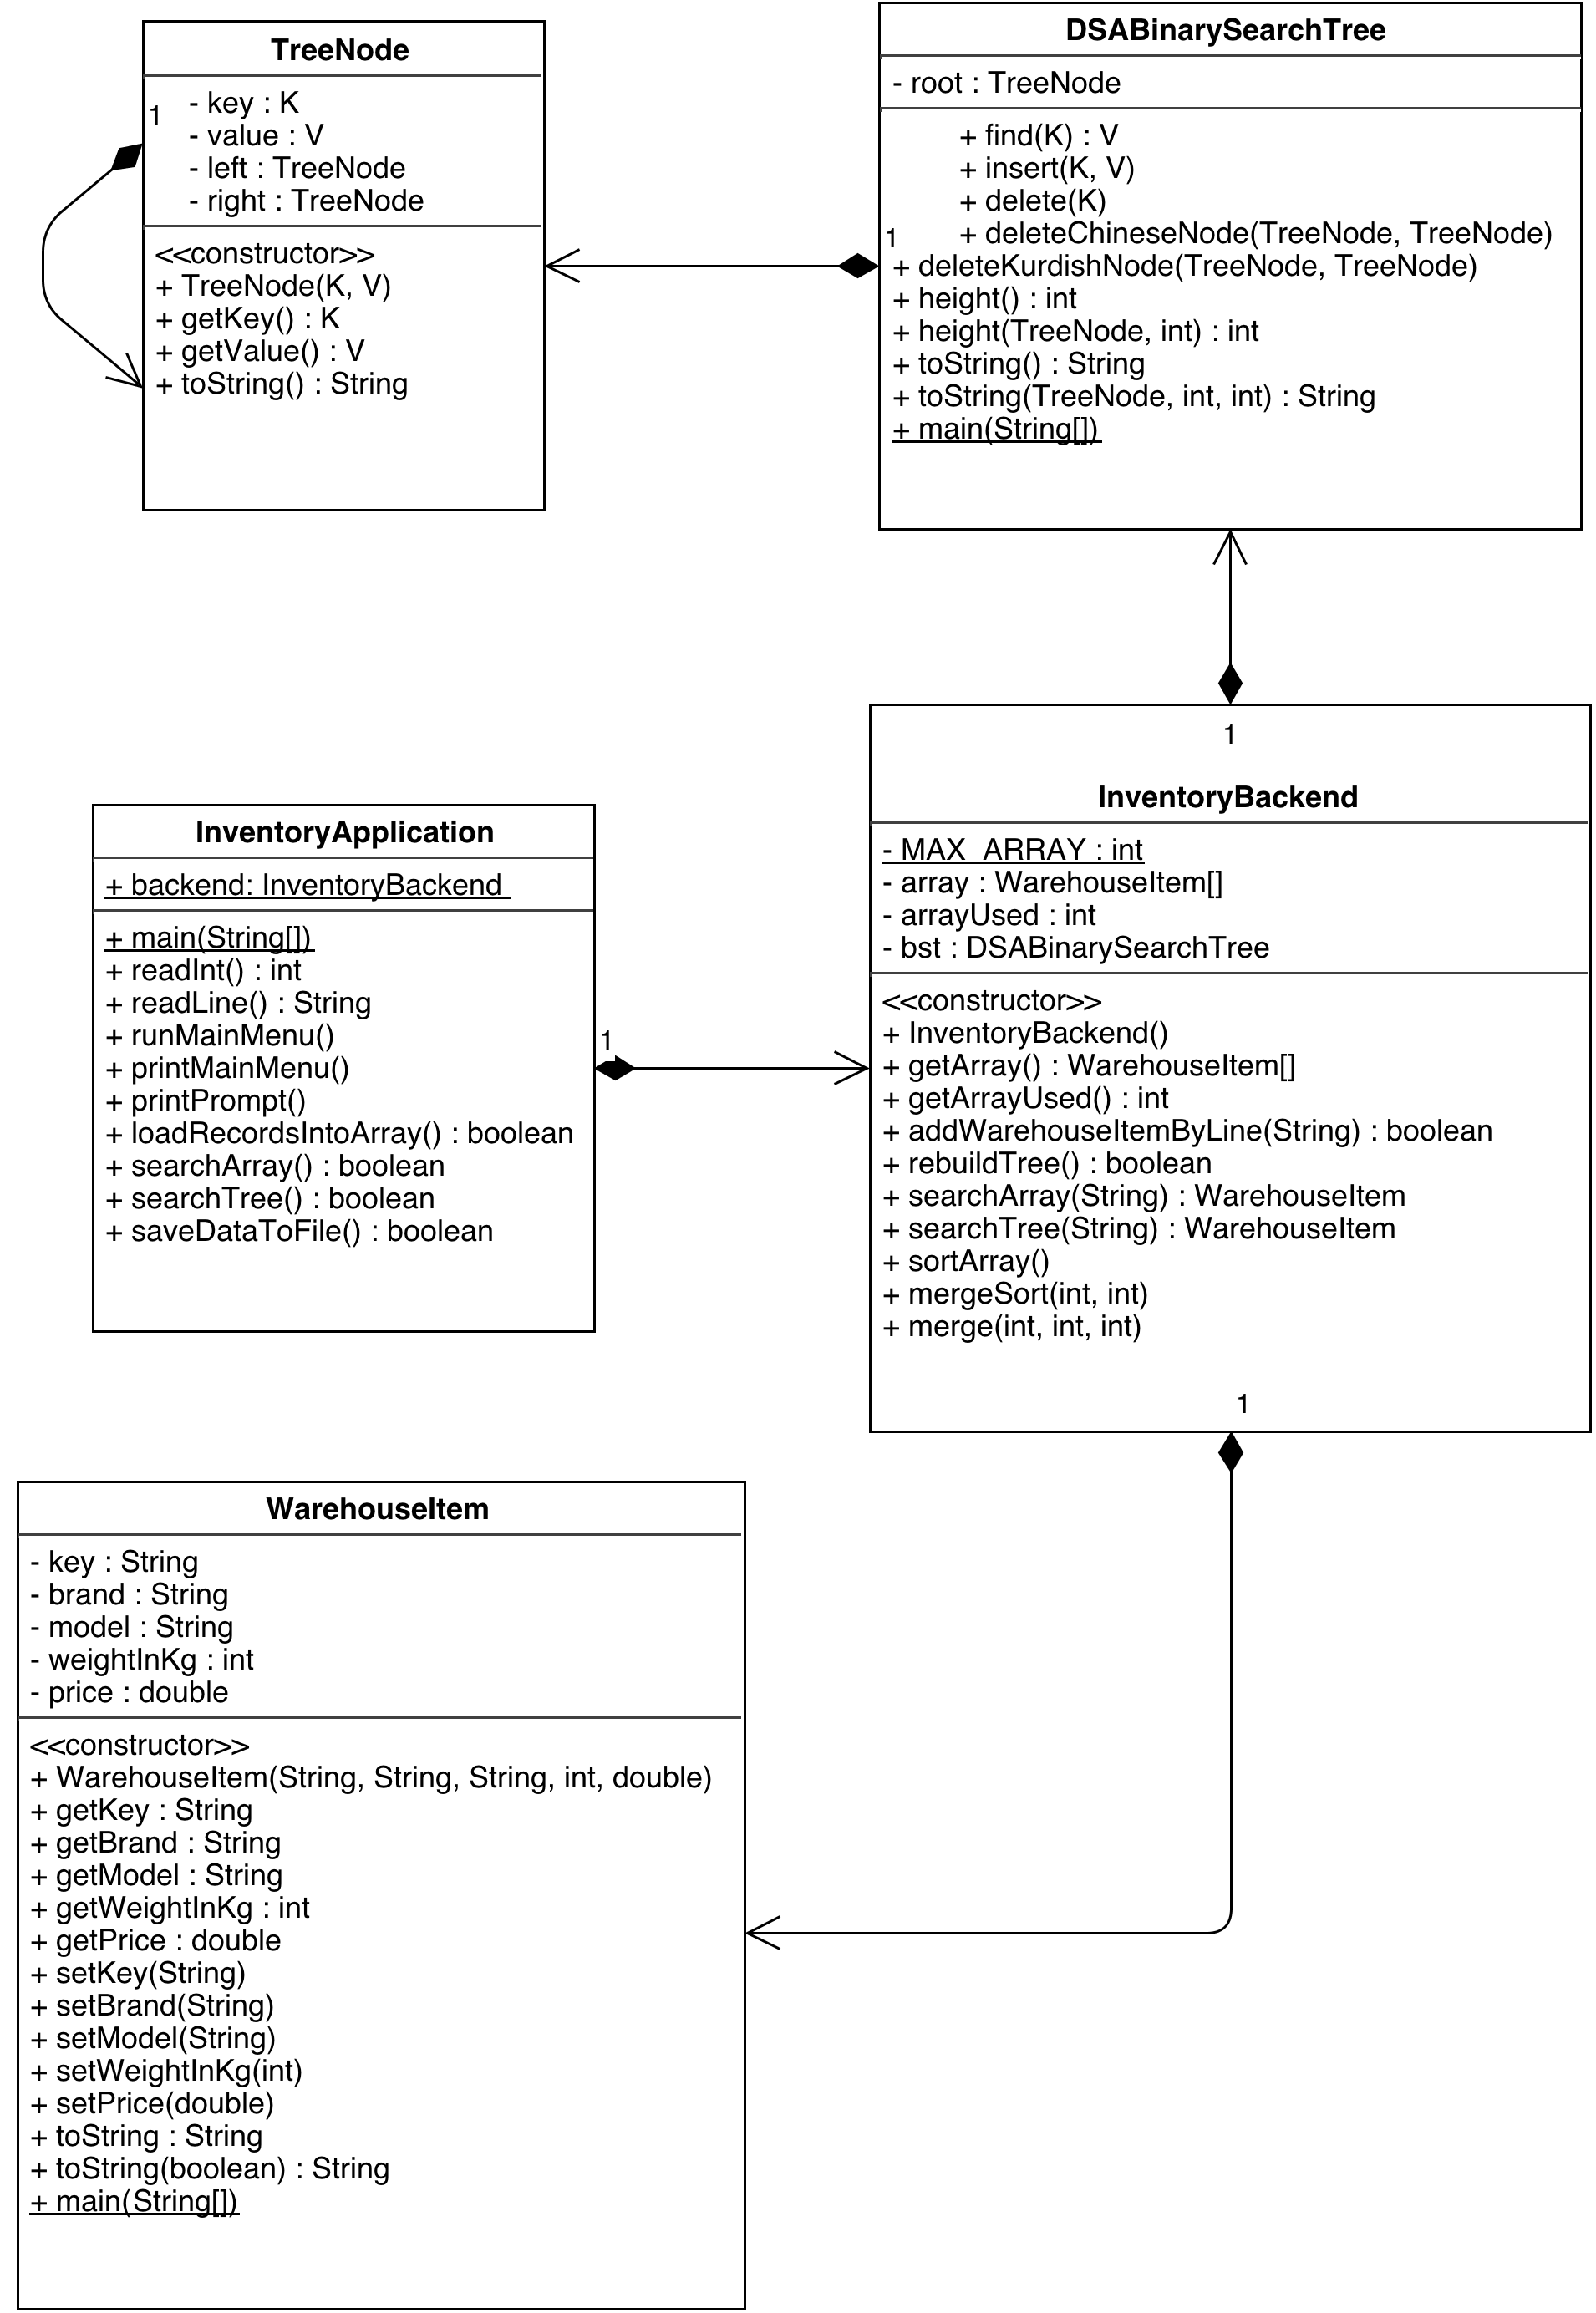
\includegraphics[width=15cm]{umldiagram.png}

\end{document}
